\section{General Implementation}
The game is created as a web page that uses WebGL to load the game, as such it needs to run on a web server so it can be accessed from the internet. The web server used in this project is Apache running on Debian Linux, the Apache server has been extended with the Wsgi module such that it can run Python. The server needs to run Python because the website uses the Django framework to serve the content.

\begin{figure}[ht]
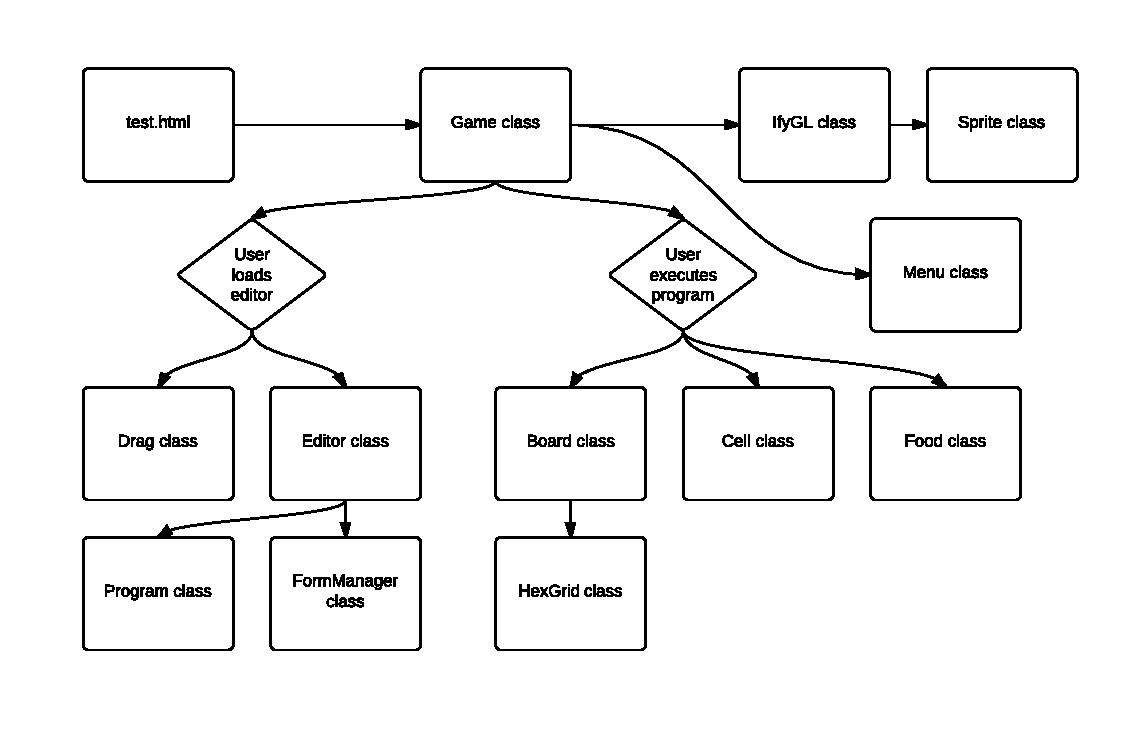
\includegraphics[width=\textwidth]{img/Program_flow.pdf}
\caption{The general flow of the program.}
\label{fig:programflow}
\end{figure}

\autoref{fig:programflow} shows the general flow of the program, the rest of this section will explain the flow in more detail.\newline

When a user opens the game in a browser, the first thing that is loaded is the \texttt{test.html} document. The \texttt{test.html} page loads all the JavaScript scripts that run the program, as well as defining the HTML5 canvas and the styles of the page. At the end of the \texttt{test.html} page, the game is loaded with the lines: 

\begin{lstlisting}
g = new Game();
g.init();
\end{lstlisting}

These commands first run the \texttt{Game} function in the class of the same name, which in turn starts by loading the IfyGL class which handles the WebGL initialization and drawing of sprites. Then the \texttt{init} function of the Game class is run, this function loads the sprites used in the menu and game, it also loads mouse events and the menu itself. At the end of the function, the draw loop is specified such that the game is redrawn every 17 milliseconds, giving a frame rate of 60 fps.
When this is done, the game has been loaded and draws the menu, which the user can use to navigate through the game.\newline

Using the menu, a user can start a game, which loads the Editor and Drag classes. The Editor class then loads a new program in the Program class and the form manager in the FormManager class. The Editor class also loads sprites used in the editor. When the user is ready to execute the program they have written, they can choose to load the game board. This loads the Board, Cell, and Food class. All navigation is handled by states that are set, the Game class and the Menu class check for states and load the appropriate content based on these.